\chapter{The Fundamental Theory For Spectral Methods}
\label{Chapter_2}
    
	\vspace{0.3cm}
	In this chapter, we will present the elements necessary to solve partial differential equations using spectral methods given as follows
	\begin{align}
	\label{general_problem}
	\left \lbrace \begin{array}{ll}
		&\frac{\partial u}{\partial t} = \mathcal{L} u, \hspace{3mm} x \in I, \hspace{3mm} t > 0,\\
		\\
		&u(x, 0) = g(x), \hspace{9mm} x \in I, 
		\end{array}  \right .
	\end{align}
	where $u$ is defined in some Hilbert space $\mathcal{H}$, with initial condition $g(x) \in \mathcal{H}$ and $\mathcal{L}$ is some spatial differential operator, which allows us to represent the previous problem in another whose solution $u$ will be given by a linear combination of already known functions. \\
	
	To do this, suppose that $\mathcal{H}$ is a separable Hilbert space with the inner product $\langle \cdot, \cdot \rangle$. Therefore, we can represent the function $u$ in terms of a known orthonormal base of $\mathcal{H}$, which we will denote as $\{\phi_k \}_{k \in I}$, given as follows 
	\begin{align*}
		\displaystyle u = \sum_{k \in I} \langle \phi_k, u \rangle \phi_k.
	\end{align*}
	
	There is a wide variety of families of base functions, which define different spectral methods. In this chapter, we will consider the well-known Fourier basis given by
	\begin{align}
		\label{base_phi}
		\phi_n (x) = e^{inx}.
	\end{align}
	that form an orthogonal set with the standard interior product $L^2$ in the interval $(0, 2 \pi)$, that is,
	\begin{align}
	\label{ortho_phi}
	\displaystyle \int_{0}^{2\pi} \phi_k (x) \overline{\phi_l (x)} dx = 2 \pi \delta{kl} = \left \lbrace \begin{array}{ll}
	0 \hspace{3mm} &\text{if} \hspace{3mm} k \neq l, \\
	2 \pi &\text{if} \hspace{3mm} k = l.
	\end{array}  \right.
	\end{align}
	
	We will denote as $B = span\{e^{inx}: |n| \leq \infty \}$ the set containing the Fourier bases. Therefore, we can define the Fourier series $F[u]$ for $u(x) \in L^2 [0, 2\pi]$ as follows 
	\begin{equation}
	\label{fourier_series}  
		F[u] \equiv \displaystyle \sum_{ |n| \leq \infty} \hat{u}_{n} e^{inx},
	\end{equation}
	where
	\begin{align}
	\label{coeff_fourier}
	\hat{u}_n = \frac{1}{2 \pi} \displaystyle \int_{0}^{2 \pi} u(x) e^{-inx} dx, \hspace{3mm}  k = 0, \pm 1, \pm 2, \dots.
	\end{align}
	which is known as the classical continuous series of trigonometric polynomials, where $\hat{u}_{n}$ are the Fourier coefficients. \\
    
    It is important noted that the integrals in (\ref{coeff_fourier}) exist if $u$ is Riemann-integrable, i.e., if $u$ is bounded and piecewise continuous in $(0, 2 \pi)$. More generally, the Fourier coefficients are defined for any function that is integrable in the Lebesgue sense. Also the relation (\ref{coeff_fourier}) associates with $u$ a sequence of complex numbers called the Fourier transform of $u$. It is possible as well to introduce a Fourier cosine transform and a Fourier sine transform of $u$, respectively, through the formulas
    \begin{align}
    \label{coeff_a_n}
    	a_n = \frac{1}{2 \pi} \displaystyle \int_{0}^{2 \pi} u(x) \cos(nx) dx, \hspace{3mm}  n = 0, \pm 1, \pm 2, \dots,
    \end{align}
    and
    \begin{align}
    \label{coeff_b_n}
    	b_n = \frac{1}{2 \pi} \displaystyle \int_{0}^{2 \pi} u(x) \sin(nx) dx, \hspace{3mm}  n = 0, \pm 1, \pm 2, \dots.
    \end{align}
    The three Fourier transforms of $u$ are related by the formula $\hat{u}_n = a_n - ib_n$ for $n = 0, \pm 1, \pm 2, \dots$. Moreover, if $u$ is a real valued function, $a_n$ and $b_n$ are real numbers, and $\hat{u}_{-n} = \hat{u}_n$. \\
	
	Based on the above, we will present two tools to build the methods that will be used in Chapter \ref{Chapter_3}, and that will be developed independently in the following two sections. In the first section, we will see that with the continuous Fourier expansion we can define a projection operator on a space of finite dimension that will allow us to approximate a function and its derivatives. In the second and last section, due to the complexity of the calculation of the previous integrals, we will see that it is possible to use quadrature rules to approximate them, and thus define an interpolation operator that will give us a discrete representation for a function and its derivatives.
	
	For these two operators, at the end of each section we will discuss the factors that determine the behavior of the series when used to approximate smooth functions, showing how fast they approach, when, and in what sense they are convergent.
	
	\newpage
	\section{Projection Operator: Continuous Fourier Expansion}
	\vspace{0.2cm}
		
	We define the projection operator denoted as $\mathcal{P}_N$ as the truncated Fourier series, i.e.,
	\begin{equation}
	\label{proyection_operator}
		\mathcal{P}_N u(x) \equiv  \displaystyle \sum_{ |n| \leq \frac {N}{2}} \hat{u}_{n} e^{inx}.
	\end{equation}	
	We will denote to $\hat{B}_N$ as the finite subset of $B = span\{e^{inx}: |n| \leq \infty \}$ on which it is projected the function, represented as follows
	\begin{align*}
		\hat{B}_{N} = span \left\{e^{inx}: |n| \leq \frac {N}{2} \right\},\hspace{0.2cm} dim(\hat{B}_{N}) = N + 1.
	\end{align*}
	Then by the orthogonality relation (\ref{ortho_phi}), it can be seen that for $u(x) \in L^2 [0, 2\pi]$
	\begin{align*}
		\langle \mathcal{P}_N u, v \rangle = \langle u, v \rangle, \hspace{3mm} \forall v \in S_N.
	\end{align*}
	This shows that $\mathcal{P}_N u$ is the orthogonal projection of $u$ upon the space of the trigonometric polynomials of degree $N$.\\
	
	Equivalently, $\mathcal{P}_N u$ is the closest element to $u$ in $\hat{B}_N$ with respect to the inner product
	\begin{align*}
		\langle u, v \rangle = \displaystyle \int_{0}^{2 \pi} u(x) \overline{v(x)} dx,
	\end{align*}
	and this also defines the norm
	\begin{align}
	\label{L2_dot}
		\| u \|^2 = \displaystyle \int_{0}^{2 \pi} |u(x)|^2 dx.
	\end{align}
	
	A full characterization of the functions for which the Fourier series is convergent is the framework of Lebesgue integration for convergence in mean. This convergence can be defined in $L^2 (0, 2 \pi)$ (square-integrable functions), also is a complex Hilbert space with inner product defined by (\ref{L2_dot}). Then for $u \in L^2 (0, 2 \pi)$ the Fourier series $F(u)$ given by (\ref{fourier_series}) is said to be convergent in mean (or $L^2$-convergent) to $u$ if
	\begin{align}
		\label{L2_mean}
		\displaystyle \int_{0}^{2 \pi} |u(x) - \mathcal{P}_N u(x) |^2 dx \rightarrow 0, \hspace{2mm} \text{as} \hspace{2mm} N \rightarrow \infty,
	\end{align}
	
	Then the Functions in $L^2 (0, 2 \pi)$ can be characterized in terms of their Fourier coefficients, according to the Riesz theorem, in the following sense. If $u \in L^2 (0, 2 \pi)$, then its Fourier series converges to $u$ in the sense of (\ref{L2_mean}), and by Parseval's identity show us that
	\begin{align}
	\label{parseval}
		\| u \|^2 = 2 \pi \displaystyle \sum^{\infty}_{-\infty} |\hat{u}_n|^2.
	\end{align}
	Conversely, if for any complex sequence $\{\hat{u}_n \}$, $n = 0, \pm 1, \dots $, and $\sum^{\infty}_{n=-\infty} |\hat{u}_n|^2 < \infty$, there exists a unique function $u \in L^2 (0, 2 \pi)$ such that its Fourier coefficients are precisely the $\hat{u}_n$$'$s for any $n$. Thus, for any function $u \in L^2 (0, 2 \pi)$ can be written as
	\begin{align}
		u = \displaystyle \sum^{\infty}_{n=-\infty} \hat{u}_n \phi_n.
	\end{align}
	
	The Riesz theorem states that the finite Fourier transform is an isomorphism between $L^2 (0, 2\pi)$ and the space $l^2$ of complex sequences $\{\hat{u}_n \}$, $n = 0, \pm1, \pm2, \dots$, such that $\sum^{\infty}_{n=-\infty} |\hat{u}_n|^2 < \infty$. The above can be summed up in the following theorem. 
	
	\begin{teor}
		 If the sum of squares of the Fourier coefficients is bounded
		\begin{align*}
			\displaystyle \sum_{ |n| \leq \infty} |\hat{u}_n|^2 < \infty
		\end{align*}
		then the truncated series converges in the $L^2$ norm
		\begin{align*}
			\|u -  \mathcal{P}_N u \|_{L^2 [0, 2\pi]} \rightarrow 0 \hspace{0.5cm} \text{as} \hspace{0.5cm} N \rightarrow \infty.
		\end{align*}
		If, moreover, the sum of the absolute values of the Fourier coefficients is bounded
		\begin{align*}
			\displaystyle \sum_{ |n| \leq \infty} |\hat{u}_n| < \infty
		\end{align*}
		then the truncated series converges uniformly 
		\begin{align*}
			\|u -  \mathcal{P}_N u \|_{L^{\infty} [0, 2\pi]} \rightarrow 0 \hspace{0.5cm} \text{as} \hspace{0.5cm} N \rightarrow \infty. 
		\end{align*}
	\end{teor}
	
	Note that if the truncated sum converges implies that the error is dominated by the tail of the series, i.e.,
	\begin{align*}
		\|u -  \mathcal{P}_N u \|^2_{L^2 [0, 2\pi]} = 2 \pi	\displaystyle \sum_{ |n| > \frac{N}{2} } |\hat{u}_n|^2,
	\end{align*}	
	and	
	\begin{align*}
		\|u -  \mathcal{P}_N u \|_{L^{\infty} [0, 2\pi]} \leq 
		\displaystyle \sum_{|n| > \frac{N}{2}} |\hat{u}_n|. 
	\end{align*}
	Thus, the error committed by replacing $u(x)$ with its $N$th-order Fourier series depends solely on how fast the expansion coefficients of $u(x)$ decay. \\
	
	To appreciate this, suppose that $u(x) \in L^2_p [0, 2 \pi]$ and that its derivative $u'(x) \in L^2_p [0, 2\pi]$, where the subscript $p$ indicate that the function is periodic. then for $n \neq 0$ we have to
	\begin{align*}
		2\pi \hat{u}_N &= \displaystyle \int_{0}^{2\pi} u(x) e^{-inx} dx \\
		&= - \frac{1}{in} (u(2\pi) - u(0)) - \frac{1}{in} \displaystyle \int_{0}^{2\pi} u'(x) e^{inx} dx, 
	\end{align*}
	therefore
	\begin{align*}
		|\hat{u}_N| \propto \frac{1}{n}.
	\end{align*}
	
	In general, if for $u(x)$ and its derivatives $(m - 1)$, and its periodic extensions are all continuous, and also if its derivative $m$th is measurable at $[0, 2 \pi]$, also known in the literature as the regularity of the function, in this particular case in $L^2_p$, we have to $\forall n \neq 0$, repeating the previous procedure successively, the behavior of Fourier coefficients $\hat{u}_n$ of $u(x)$ is similar, i.e.,
	\begin{align*}
		|\hat{u}_n| \propto \left(\frac{1}{n}\right)^m.
	\end{align*}
	
	 This is known as spectral convergence, which means that the smoother the function, the series converges faster.\\
	 
	 This result is important since it will allow us to investigate the convergence rate of the methods, which we will define in detail later. Therefore, we will focus on periodic functions expanded in Fourier series since its rapid decay of the coefficients implies that the Fourier series truncated after just a few more terms represents an exceedingly good approximation of the function. However, in practice, this decay is not exhibited until there are enough coefficients to represent all the essential structures of the function but in general, functions can be described both through their values in physical space and through their coefficients in transform space. The following examples illustrate the previous results. \\
	 
	\begin{example}
	    Consider the function $u(x) \in C^{\infty} [0, 2 \pi]$ given by
    	\begin{align}
    		\label{Example1} 
    	    u(x) = \frac{1}{5 - 4 \cos(x)}   
    	\end{align}
    	with its expansion coefficients
    	\begin{align*}
    	     \hat{u}_{n} = \frac{2^{-|n|}}{3}.
    	\end{align*}
    
    	In Figure \ref{fig1} we can clearly observe the convergence of the Fourier series and that in addition, the convergence of the approximation is almost uniform. This is due to the periodicity of the function and its derivatives.
    	
    	\begin{figure}[H]
        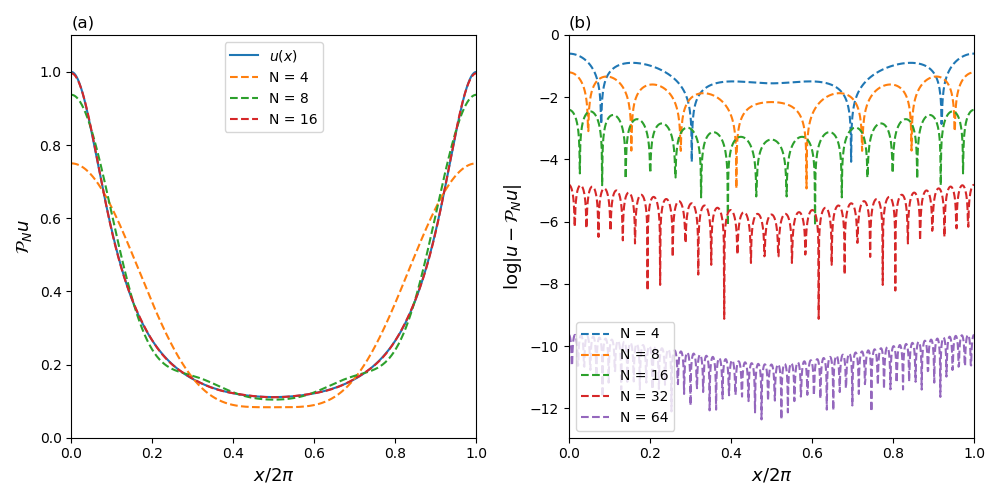
\includegraphics[width=\textwidth]{preliminaries/figures/example21.png}
        \caption{(a) Continuous Fourier series approximation of the equation (\ref{Example1}). (b) The Pointwise error of approximation.}
        \label{fig1}
        \end{figure}
	\end{example} 
	
	\begin{example}
	    The expansion coefficients of the function
    	\begin{align}
    		\label{Example2} 
    	    u(x) = \frac{\pi}{2} \sin(\frac{x}{2})
    	\end{align}
    	are given by
    	\begin{align*}
    	     \hat{u}_{n} = \frac{1}{(1 - 4n^2)}.
    	\end{align*}
    	
    	Note that is infinitely differentiable in $[0, 2 \pi]$, but $u'(0) \ne u' (2 \pi)$. In Figure \ref{fig2} we can see that the convergence is much slower than in the Example \ref{Example1}, as expected	
    	\begin{figure}[H]	
        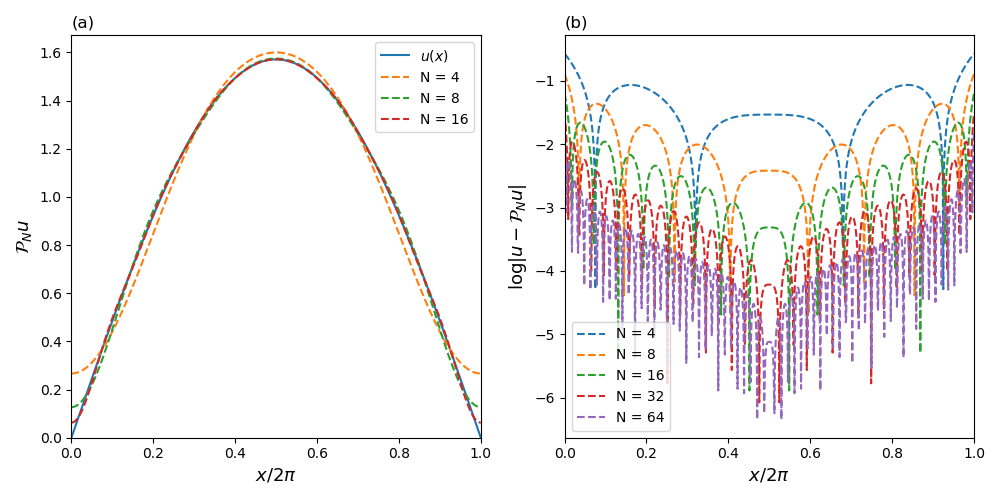
\includegraphics[width=\textwidth]{preliminaries/figures/example22.png}
        \caption{(a) Continuous Fourier series approximation of the equation (\ref{Example2}). (b) The Pointwise error of approximation for increasing resolution.}
        \label{fig2}
    	\end{figure}
	\end{example} 
	
	\subsection{Differentiation of the Continuous Expansion}

	To find solutions of partial differential equations using the spectral methods, in addition to approximating a function $u(x)$ by the finite Fourier series $\mathcal{P}_N u$, we also need to obtain its derivatives. Due to the linearity of the derivative and that these functions are exponential, we can easily obtain the derivatives of $\mathcal{P}_N u$ by simply differentiating the basis functions term by term. Therefore, if we have the following series truncated \\
 	\begin{align*}
   		\mathcal{P}_N u(x) =  \displaystyle \sum_{ |n| \leq \frac {N}{2}} \hat{u}_{n} e^{inx},
   	\end{align*}
    from this, we can get
   	\begin{align*}
   		\frac{d^q}{dx^q} \mathcal{P}_N u(x) = \displaystyle \sum_{ |n| \leq \frac {N}{2}} \hat{u}_{n} \frac{d^q}{dx^q} e^{inx} = \displaystyle \sum_{ |n| \leq \frac {N}{2}} (in)^q \hat{u}_{n}e^{inx}.
   	\end{align*}
    Therefore the projection and differentiation operators commute, i.e.,
    	\begin{align*}
    	\mathcal{P}_N \frac{d^q}{dx^q} u = \frac{d^q}{dx^q}\mathcal{P}_N u.
    	\end{align*}
    This property implies that for any differentiation operator $\mathcal{L}$ with constant coefficients,	
    	\begin{align*}
    	\mathcal{P}_N \mathcal{L} (I - \mathcal{P}_N)u
    	\end{align*}
     vanishes, which known as the truncation error. Thus, the Fourier approximation to the equation $u_t = \mathcal{L}u$ is exactly the projection of the analytic solution. 

    \subsection{Approximation theory for Continuous Expansion.}
    
    The behavior of the functions and their derivatives that we have shown is relevant when the solutions of the differential equations are approximated using spectral methods since it allows us to investigate how fast and precise they can be. In this subsection, we will present these properties based in \cite{gottlieb2007} as detailed as possible some useful results for our main objective regarding the analysis of the projection operator already defined above. \\
    
    When using the Fourier approximation to discretize the spatial part of the equation
    \begin{align*}
        u_t = \mathcal{L}u,
    \end{align*}
    it is important that our approximation, both to $u$ and to $\mathcal{L}u$, be accurate,i.e., we must consider not only the difference between $u$ and $\mathcal{P}_N u$ if not also the distance between $\mathcal{L} u$ and $\mathcal{L} \mathcal{P}_N u$, measured in an appropriate norm. This is because the actual rate of convergence is determined by the truncation error    
    \begin{align*}
    	\mathcal{P}_N \mathcal{L} (I - \mathcal{P}_N)u.
    \end{align*}
   	Thus, the error is determined not only by the behavior of the Fourier approximations of the function but also of its derivatives, as we have seen previously. Therefore, the Sobolev $q$-norm denoted by $H^q_p [0, 2\pi]$, It is appropriate to estimate the truncation error since it measures the smoothness of the derivatives and the function. This norm is defined as follows
    \begin{align}
    \label{sobolev_norm}
    	 \|u\|^2_{H^q_p [0, 2\pi]} = \displaystyle \sum^{q}_{m=0} \int^{2\pi}_{0} \left| u^m (x) \right|^2 dx.
    \end{align}
    The subscript $p$ indicates the fact that all functions are periodic. By substituting the Fourier expansion for each derivative in (\ref{sobolev_norm}), the Sobolev norm can be written as
    	\begin{align*}
    	    \|u\|^2_{H^q_p [0, 2\pi]} = 2\pi \displaystyle \sum^{q}_{m=0} \sum_{|n| \leq \infty} |n|^{2m} |\hat{u}_n|^2 = 2\pi \sum_{|n| \leq \infty} \left(\sum^{q}_{m=0} |n|^{2m} \right) |\hat{u}_n|^2,
    	\end{align*}
    where the interchange of the summation is allowed provided $u(x)$ has sufficient smoothness. \\
    
   Before starting the analysis, without loss of generality, we first consider the continuous Fourier series given by
        \begin{align*}
            \displaystyle \mathcal{P}_{2N} u(x) = \sum_{|n| \leq N} \hat{u}_n e^{in x}.
        \end{align*}
    The first important result is the estimate in $L^2$ for the distance between $u$ and its trigonometric approximation $\mathcal{P}_{2N} u$, which shows everything we've seen previously. 
    \\
    \begin{teor}
    \label{estimating_error_PN_L2}	
    For any $u(x) \in H_p^r [0, 2\pi]$, there exists a positive constant $C$, independent of $N$, such that
        \begin{align*}
    	    \|u - \mathcal{P}_{2N} u \|_{L^2 [0, 2\pi]} \leq C N^{-q} \|u^{(q)}\|_{L^2 [0, 2\pi]},
    	\end{align*}
    provided $0 \leq q \leq r$.
    \end{teor}
    \begin{proof}	
    By Parseval’s identity given by (\ref{parseval}) we get
    	\begin{align*}
    	    \|u - \mathcal{P}_{2N} u \|^2_{L^2 [0, 2\pi]} = 2\pi \displaystyle \sum_{|n| > N} |\hat{u}_n|^2.
    	\end{align*}
    We rewrite this summation as follows
    	\begin{align*}
    	    \displaystyle \sum_{|n| > N} |\hat{u}_n|^2 &= \sum_{|n| > N} \frac{n^{2q}}{n^{2q}} |\hat{u}_n|^2 \\
    	    &\leq N^{-2q} \sum_{|n| > N} n^{2q} |\hat{u}_n|^2 \\
    	    &\leq N^{-2q} \sum_{|n| \geq 0} n^{2q} |\hat{u}_n|^2 \\
    	    &= \frac{1}{2\pi} N^{-2q} \|u^{(q)}\|^2_{L^2 [0, 2\pi]}.
    	\end{align*}
    Putting all the above together and taking out the square root, we get our result.
	\end{proof}
    
    \noindent Note that the smoother the function, the larger the value of $q$ and therefore, the better the approximation, as seen before. Now let's notice the following. Suppose that $u(x)$ is analytical, so we have to
    	\begin{align*}
    		 u^{(q)} = \displaystyle 
    		 \sum_{ |n| \leq \infty} (in)^q \hat{u}_{n}e^{inx}.
    	\end{align*}
    Since $u^{(q)} \in W^q_p$, and by (\ref{parseval})
        \begin{align*}
            \|u^{(q)}\|_{L^2 [0, 2\pi]} = \sum_{ |n| \leq \infty} |n|^{2q} |\hat{u}_{n}|^2 \leq C q! \sum_{ |n| \leq \infty} |\hat{u}_{n}|^2 \leq C q! \| u \|_{L^2 [0, 2\pi]},
        \end{align*}
    and so by the previous theorem
        \begin{align*}
            \|u - \mathcal{P}_{2N} u \|_{L^2 [0, 2\pi]} \leq  N^{-q} \|u^{(q)}\|_{L^2 [0, 2\pi]} \leq C \frac{q!}{N^{q}} \| u \|_{L^2 [0, 2\pi]}.
        \end{align*}
    Using Stirling’s formula, $q! \sim q^q e^{-q}$, and assuming that $q \propto N$, we obtain
        \begin{align*}
            \|u - \mathcal{P}_{2N} u \|_{L^2 [0, 2\pi]} \leq \sim C \left(\frac{q}{N}\right)^q e^{-q} \| u \|_{L^2 [0, 2\pi]} \sim K e^{-c N} \| u \|_{L^2 [0, 2\pi]}.
        \end{align*}
    Thus, for an analytic function, its spectral convergence is exponential convergence. \\
    
    We must not forget that the theory we have previously presented is with the assumption that the functions and their derivatives are all periodic. But it is possible to do a similar analysis considering some other class of functions, such as functions that vanish at the borders. However, these kinds of functions belong to spaces very similar to those we have studied, and it is possible to use the same results.  
	
	\newpage
	\section{Interpolation Operator: Discrete Fourier Expansion}
    
    The continuous Fourier series method requires the evaluation of the coefficients
    \begin{align}
        \hat{u}_n = \displaystyle \frac{1}{2\pi} \int_{0}^{2\pi} u(x) e^{-inx} dx.
    \end{align}
    In general, these integrals cannot be computed analytically, and one resorts to the approximation of the Fourier integrals by using quadrature formulas. This procedure defines a discrete transform between the set of values of $u$ at the quadrature points and the set of approximate, or discrete, coefficients. The finite series defined by the discrete transform is actually the interpolate of $u$ at the quadrature nodes. If the properties of accuracy (in particular the spectral accuracy) are retained by replacing the finite transform with the discrete transform, then the interpolant series can be used instead of the truncated series to approximate functions. Also, quadrature formulas differ based on the exact position of the grid points, and the choice of an even or odd number of grid points results in slightly different schemes.
    
    \subsection{The Even Expansion}
    
    Define an equidistant grid, consisting of an even number $N$ of gridpoints $x_j \in [0, 2\pi)$, defined by
	\begin{align*}
        x_j = \frac{2 \pi j}{N} , \hspace{0.5cm} j\in [0, \cdots , N -1]. 
    \end{align*}
    The trapezoidal rule yields the discrete Fourier coefficients $\widetilde{u}_n$, which approximate the continuous Fourier coefficients $\hat{u}_n$ given as follows    
    \begin{align}
        	\widetilde{u}_n = \frac{1}{N}  \displaystyle \sum_{j = 0}^{N - 1} u(x_j) e^{-in x_j}.
    \end{align}
	The difference between the continuous and the discrete approximation is very clear since here we only need precision in the points $ x_j $. This may somehow be an advantage in the numerical calculation because in some cases it is possible to obtain the same order of precision, as shown in the following theorem when trigonometric polynomials are involved, the trapezoidal quadrature rule is a very natural approximation. \\
	
	\begin{teor}
	\label{Exactness_Even}	
	For the points $x_j$ defined as above, the quadrature formula
    \begin{align*}
         \frac{1}{2\pi}\displaystyle \int^{2\pi}_{0} f(x) dx = \frac{1}{N} \displaystyle \sum^{N-1}_{j=0} f(x_j), 
    \end{align*}
    is exact for any trigonometric polynomial $f(x) = e^{inx}$ , $|n| < N$.
    \end{teor}
	\begin{proof}
	Given a function $f(x) = e^{in x}$, It is easy to observe that
	
    \begin{align*}
        \frac{1}{2\pi}\displaystyle \int^{2\pi}_{0} f(x) dx =  \left \lbrace \begin{array}{ll}
    	1 \hspace{3mm} & \text{if } n = 0, \\
    	0 \hspace{3mm} & \text{otherwise.}
    	\end{array}  \right . 
    \end{align*}

	\noindent On the other hand,    
    \begin{align*}
        \frac{1}{N}  \displaystyle \sum_{j = 0}^{N - 1} f(x_j) &= \frac{1}{N}  \displaystyle \sum_{j = 0}^{N - 1} e^{in (\frac{2\pi j}{N})} \\
        &= \frac{1}{N}  \displaystyle \sum_{j = 0}^{N - 1} q^j
    \end{align*}
    where $q = e^{i \frac{2\pi n}{N}}$. If $n$ is an integer multiple of $N$ , i.e., $n = m N$, then, we have to
    \begin{align*}
    	\displaystyle \frac{1}{N} \sum^{N-1}_{j=0}  e^{i Nm (\frac{2\pi j}{N})} = \frac{1}{N} \sum^{N-1}_{j=0}  e^{i(2\pi j m)} = 1
    \end{align*} 
	Otherwise, 
	\begin{align*}
		\displaystyle \frac{1}{N} \sum^{N-1}_{j=0} q^j = \frac{q^{N} - 1}{q - 1} = 0
	\end{align*}
	Thus, the quadrature formula is exact for any function of the form $f(x) = e^{inx}$, $|n| < N$.
	\end{proof}

	Moreover, we can see that the quadrature formula is exact for $f(x) \in \hat{B}_{2N-2}$ where $\hat{B}_N$ is defined as before. Then using the trapezoid rule, the discrete Fourier coefficients become
	\begin{align}
	\label{coeficients_IN}
	    \widetilde{u}_n = \frac{1}{N \widetilde{c}_n}  \displaystyle \sum_{j = 0}^{N - 1} u(x_j) e^{-in x_j},
	\end{align}
	where we introduce the coefficients
	\begin{align}
	\label{constants_IN}	
	    \widetilde{c}_n = \left \lbrace \begin{array}{ll}
	    2  \hspace{0.25cm}\text{if} & |n| =  N/2, \\
	    \\
	    1  \hspace{0.25cm} \text{if} & |n| < N/2.
	\end{array}  \right .
	\end{align}

	\noindent These relations define a new projection of $u$
	\begin{equation}
	\label{collocation_operator_even}
		\mathcal{I}_N u(x) =  \displaystyle \sum_{ |n| \leq \frac {N}{2}} \widetilde{u}_n e^{inx}
	\end{equation}
	This is the complex discrete Fourier transform, based on an even number of quadrature points. From the above, we can see that
	\begin{align*}
	    \widetilde{u}_{-N/2} = \widetilde{u}_{N/2},
	\end{align*}
	so we have exactly $N$ independent Fourier coefficients, corresponding to the $N$ quadrature points. As a consequence, $\mathcal{I}_N \sin( \frac{N}{2} x) = 0$, so that the function $\sin( \frac{N}{2} x)$ is not represented in the above expansion. Therefore, the space $\hat{B}_N$ does not include $\sin( \frac{N}{2} x)$, and the correct space must be as follows
	\begin{align*}
	    \widetilde{B}_N = span\left\{\left(\cos(nx), \hspace{0.2cm} 0 \leq n \leq \frac{N}{2} \right)\cup  \left(\sin(nx), \hspace{0.2cm} 1 \leq n \leq \frac{N}{2} - 1 \right)\right\},
	\end{align*}
	which has dimension dim$(\widetilde{B}_N) = N$.\\
	
	\noindent In the same way, as in the previous subsection using the discrete expansion for Examples \ref{Example1} and \ref{Example2}, we can observe the same behavior as with continuous expansion, but now we have that the error at each point $x_j$ of the grid is zero.

	\begin{example}
	    Consider the $C^{\infty}_p [0, 2 \pi]$ function
    	\begin{align}
    		\label{Example4}
    	    u(x) = \frac{1}{5 - 4 \cos(x)}.
    	\end{align}
    	Its expansion coefficients are
    	\begin{align*}
    	     \hat{u}_{n} = \frac{2^{-|n|}}{3}.
    	\end{align*}
    	\begin{figure}[H]
        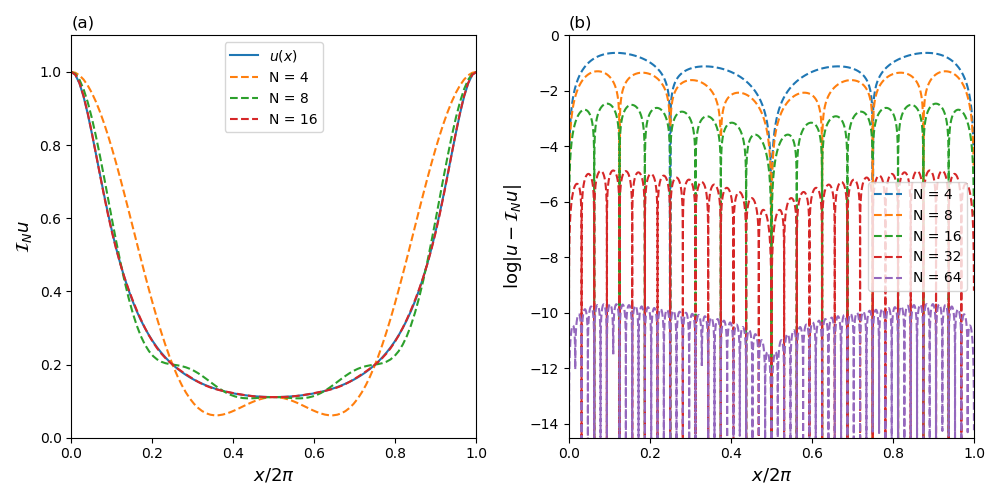
\includegraphics[width=\textwidth]{preliminaries/figures/example23.png}
        \caption{(a) Discrete Fourier series approximation of the equation (\ref{Example4}). (b) Pointwise error of approximation for increasing resolution.}
        \label{fig3}
        \end{figure}
	\end{example} 
	
	\begin{example}
	    The expansion coefficients of the function
    	\begin{align}
    		\label{Example5}
    	    u(x) = \frac{\pi}{2} \sin(\frac{x}{2}),
    	\end{align}
   		are given by
    	\begin{align*}
    	     \hat{u}_{n} = \frac{1}{(1 - 4n^2)}.
    	\end{align*}
    	\begin{figure}[H]
        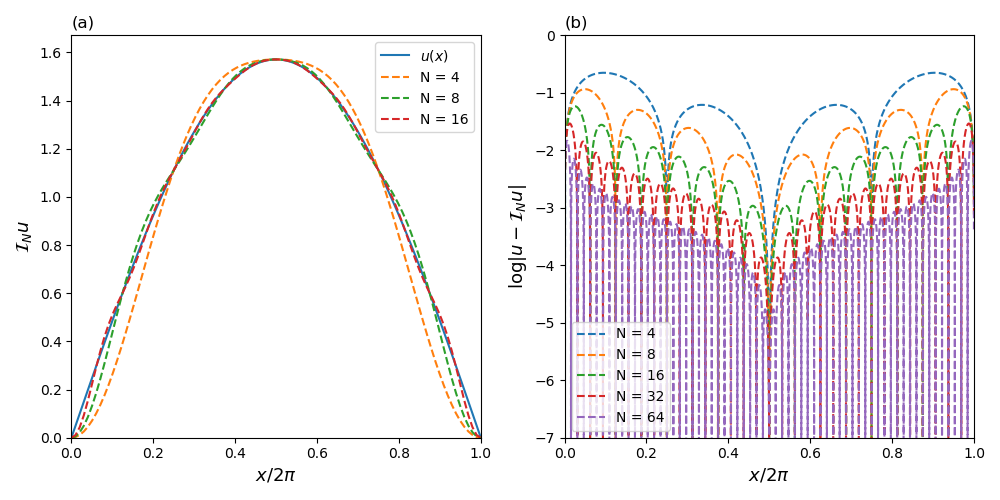
\includegraphics[width=\textwidth]{preliminaries/figures/example24.png}
        \caption{(a) Discrete Fourier series approximation of the equation (\ref{Example5}). (b) Pointwise error of approximation for increasing resolution.}
        \label{fig4}
        \end{figure}
	\end{example} 
	
	Therefore, we can see that the discrete expansion is, in fact, an interpolation operator as mentioned. This can be shown in the following theorem.\\
	
	\begin{teor}
	Let the discrete Fourier transform be defined by Equations (\ref{coeficients_IN})-(\ref{collocation_operator_even}). For any periodic function, $C^{0}_p [0, 2\pi]$, we have
	\begin{align*}
		\mathcal{I}_N u(x_j) = u(x_j), \hspace{0.3cm} \forall x_j = \frac{2 \pi j}{N} , \hspace{0.3cm} j = 0, \dots, N - 1. 
	\end{align*}
	\end{teor}

	\begin{proof}
	Substituting Equation (\ref{coeficients_IN}) into Equation (\ref{collocation_operator_even}) we obtain
	
	\begin{equation*}
    	\mathcal{I}_N u(x) =  \displaystyle \sum_{ |n| \leq \frac {N}{2}} \left(\frac{1}{N \widetilde{c}_n}  \displaystyle \sum_{j = 0}^{N - 1} u(x_j) e^{-in x_j}\right) e^{inx}.
	\end{equation*}
	Exchanging the order of the sum gives
	\begin{align}
	    \mathcal{I}_N u(x) = \displaystyle \sum_{j=0}^{N-1} u(x_j) g_j (x),
	\end{align}
	where
	\begin{align*}
	    g_j (x) &= \displaystyle \sum_{ |n| \leq \frac {N}{2}} \frac{1}{N \widetilde{c}_n} e^{in(x -x_j)}\\
	    &= \frac{1}{N} \sin\left[N \frac{x - x_j}{2} \right] \cot\left[\frac{x - x_j}{2} \right]
	\end{align*}
	by summing as a geometric series. It is easily verified that $g_j (x_i) = \delta_{ij}$\\
	\\
	We still need to show that $g_j (x) \in \widetilde{B}_N$. Clearly, $g_j (x) \in \hat{B}_N$ as $g_j (x)$ is a polynomial of degree $\leq N/2$. However, since
	
	\begin{align*}
	    \frac{1}{2} e^{-i \frac{N}{2} x_j} = \frac{1}{2} e^{i \frac{N}{2} x_j} = \frac{(-1)^j}{2},
	\end{align*}
	
	and, by convention $\widetilde{u}_{-N/2} = \widetilde{u}_{N/2}$, we do not get any contribution from the term $\sin(\frac{N}{2} x)$, hence $g_j (x) \in \widetilde{B}_N$.
	\end{proof}
	
	\subsection{The Odd Expansion}
	
	Similarly, we define a grid with an odd number of grid points as follows
	\begin{align*}
        x_j = \frac{2 \pi}{N + 1} j , \hspace{0.5cm} j\in [0, \dots , N],
    \end{align*}
    and using the trapezoidal rule we get
	\begin{align}
	\label{coefficients_JN}
        \widetilde{u}_n = \frac{1}{N + 1}  \displaystyle \sum_{j = 0}^{N} u(x_j) e^{-in x_j},
    \end{align}
    to obtain the interpolation operator
    \begin{equation}
    \label{Interpolation_operator_odd}
    	\mathcal{J}_N u(x) =  \displaystyle \sum_{ |n| \leq \frac {N}{2}} \widetilde{u}_n e^{inx}.
	\end{equation}
	
    \noindent Again as before, the quadrature formula is highly accurate. \\
    \begin{teor}
    \label{Exactness_Odd}	
    For the points $x_j$ defined as above, the quadrature formula
    \begin{align*}
         \frac{1}{2\pi}\displaystyle \int^{2\pi}_{0} f(x) dx = \frac{1}{N+1} \displaystyle \sum^{N}_{j=0} f(x_j),
    \end{align*}
    is exact for any $f(x) = e^{inx}$ , $|n| < N$, i.e., for all $f(x) \in \widetilde{B}_{2N}$.
    \begin{proof}
    	Given a function $f(x) = e^{in x}$, It is easy to observe that
    	
    	\begin{align*}
    		\frac{1}{2\pi}\displaystyle \int^{2\pi}_{0} f(x) dx =  \left \lbrace \begin{array}{ll}
    			1 \hspace{3mm} & \text{if } n = 0, \\
    			0 \hspace{3mm} & \text{otherwise.}
    		\end{array}  \right . 
    	\end{align*}
    	On the other hand,    
    	\begin{align*}
    		\frac{1}{N+1}  \displaystyle \sum_{j = 0}^{N} f(x_j) &= \frac{1}{N+1}  \displaystyle \sum_{j = 0}^{N} e^{in (\frac{2\pi j}{N+1})} \\
    		&= \frac{1}{N+1}  \displaystyle \sum_{j = 0}^{N} q^j
    	\end{align*}
    	where $q = e^{i \frac{2\pi n}{N+1}}$. If $n$ is an integer multiple of $N+1$ , i.e., $n = (N+1)m$, then we have to
    	\begin{align*}
    		\displaystyle \frac{1}{N+1} \sum^{N}_{j=0}  e^{i(N+1)m (\frac{2\pi j}{N+1})} = \frac{1}{N+1} \sum^{N}_{j=0}  e^{i (2\pi jm)} = 1
    	\end{align*}
    	 Otherwise, 
    	\begin{align*}
    		\displaystyle \frac{1}{N+1} \sum^{N}_{j=0} q^j = \frac{q^{N+1} - 1}{q - 1} = 0
    	\end{align*}
    	Thus, the quadrature formula is exact for any function of the form $f(x) = e^{inx}$, $|n| < N$.
    \end{proof}
    
    \end{teor}
    The scheme may also be expressed through the use of a Lagrange interpolation polynomial,
    \begin{align}
    \label{Lagrange_Odd}	
    	\mathcal{J}_N u(x) =  \displaystyle \sum_{j=0}^{N} u(x_j) h_j (x)
	\end{align}
	where
	\begin{align}
	    h_j (x) = \displaystyle \frac{1}{N+1} \sum_{|k| \leq \frac{N}{2}} e^{ik (x - x_j)} = \frac{1}{N + 1} \frac{\sin(\frac{N+1}{2}(x - x_j))}{\sin(\frac{x - x_j}{2})}
	\end{align}
    One easily shows that $h_j (x_l) = \delta_{jl}$ and that $h_j (x) \in \hat{B}_N $.
	
	\newpage
    \subsection{Differentiation of the discrete expansions}
    
    Similarly, as in continuous expansion, we require compute derivatives of the discrete approximation. In the following subsections, we assume that our function $u$ and all its derivatives are continuous and periodic on $[0, 2\pi]$.\\
    \\
    We consider the case of an even number of grid points. Using expansion coefficients given the values of the function $u(x)$ at the points $x_j$ , differentiating the basis functions in the interpolant yields
    \begin{align}
        \frac{d}{dx} \mathcal{I}_N u(x) = \displaystyle \sum_{|n| \leq N/2} in \widetilde{u}_n e^{inx}, \hspace{2mm} \widetilde{u}_n = \displaystyle \frac{1}{N \widetilde{c}_n} \sum_{j=0}^{N-1} u(x_j) e^{-in x_j},   
    \end{align}
    where $\widetilde{c}_n$ is given by (\ref{constants_IN}). Higher order derivatives can be obtained simply by further differentiating the basis functions.\\
    
    \noindent Similarly, for the case of an odd number of grid points
    \begin{align}
    	\frac{d}{dx} \mathcal{J}_N u(x) = \displaystyle \sum_{|n| \leq N/2} in \widetilde{u}_n e^{inx}, \hspace{2mm} \widetilde{u}_n = \displaystyle \frac{1}{N + 1} \sum_{j=0}^{N} u(x_j) e^{-in x_j},   
    \end{align} 
    The procedure for differentiating using expansion coefficients can be described as follows: first, we transform the point values $u(x_j)$ in physical space into the coefficients $\widetilde{u}_n$ in mode space. We then differentiate in mode space by multiplying  $\widetilde{u}_n$ by $in$, and return to physical space.\\
    
    There are other ways to obtain these derivatives, which may have greater advantage and be more efficient to calculate. In the literature, it can commonly find the use of differentiation matrices, for which there is a great variety. We will present some matrices that have been studied in \cite{gottlieb2007}, \cite{Canuto2012}, and we will observe the difference between the cases of an even and odd number of grid points. \\
    
    \paragraph{Differentiation Matrix.} Recall that to the case of an even number of grid points, the interpolation operator can be written as
    \begin{align*}
        \mathcal{I}_N u(x) = \displaystyle \sum^{N-1}_{j=0} u(x_j) g_j (x),
    \end{align*}
    where $g_j$ are the Lagrange interpolation polynomials given by
    \begin{align*}
        g_j (x) = \frac{1}{N} \sin\left[N \frac{x - x_j}{2} \right] \cot\left[\frac{x - x_j}{2} \right].
    \end{align*}
    Then, by differentiating the interpolation directly, it can get an approximation to the derivative of $u(x)$ at the points $x_j$ as follows
    \begin{align*}
        \displaystyle \frac{d}{dx} \mathcal{I}_N (x) \Big|_{x_l} = \sum^{N-1}_{j=0} u(x_j) \frac{d}{dx} g_j (x) \Big|_{x_l} = \sum^{N-1}_{j=0} D_{lj} u(x_j),
    \end{align*}
    where $D_{lj}$ are the differentiation matrix entries given by
    \begin{align}
    \label{matrix_DN_even}
        D_{ij} = \frac{d}{dx} g_j (x) \Big|_{x_i} = \begin{cases} \frac{(-1)^{i+j}}{2} \cot \left[ \frac{x_i - x_j}{2}\right] &   i \neq j, \\ \hspace{1mm} 0 &  i=j, \end{cases}
    \end{align}
    it is also well known that $D$ is circulant and skew-symmetric matrix. In the same way, the entries of the second order differentiation matrix $D^{(2)}$ gives us
    \begin{align}
    \label{matrix_D2N_even}
        D_{ij}^{(2)} = \frac{d^2}{dx^2} g_j (x) \Big|_{x_i} = \begin{cases} -\frac{(-1)^{i+j}}{2} \left[\sin \left[ \frac{x_i - x_j}{2}\right]\right]^{-1} &   i \neq j, \\ -\frac{N^2 + 2}{12} &  i=j. \end{cases}
    \end{align}
	
    The approximation of higher derivatives follows exactly the same route, and similarly to obtain the entries of the differentiation matrix $\widetilde{D}$ for the interpolation based on an odd number of points given by
    \begin{align}
    \label{matrix_DN_odd}
        \widetilde{D}_{ij} = \begin{cases} -\frac{(-1)^{i+j}}{2} \left[\sin \left[ \frac{x_i - x_j}{2}\right]\right]^{-2} &   i \neq j, \\ \hspace{1mm} 0 &  i=j. \end{cases}
    \end{align}

    It is also known that $\widetilde{D}$ is a circulant, skew-symmetric matrix. The advantage of this method is that the differentiation matrix takes us from physical space to physical space, and the act of differentiation is hidden in the matrix itself. \\
    
    It is interesting to observe that the differentiation operator for the interpolation based on an odd number of grid points, takes elements of $\widetilde{B}_N$ out of $\widetilde{B}_N$ and then
    \begin{align*}
    	\mathcal{I}_N \frac{d^2}{dx^2} \mathcal{I}_N \neq \left( \mathcal{I}_N \frac{d}{dx} \right)^2 \mathcal{I}_N.
    \end{align*}
	
	But for the interpolation based on an odd number of grid points the differentiation operator remain in $\hat{B}_N$ when takes elements of $\hat{B}_N$, and thus,
	\begin{align*}
		\mathcal{J}_N \frac{d^2}{dx^2} \mathcal{J}_N = \left( \mathcal{J}_N \frac{d}{dx} \right)^2 \mathcal{J}_N
	\end{align*}
    Moreover, for all values of $q$ we have
    \begin{align*}
        \widetilde{D}^{(q)} = \mathcal{J}_N \frac{d^q}{dx^q} \mathcal{J}_N = \widetilde{D}^q
    \end{align*}
	allowing us to calculate approximate high derivatives by just multiplying the $D$ matrix as many times as necessary.
    
    For the above, and for some interesting properties that we will see later about interpolation operator based on an odd number of grid points, it has been decided to use it for the study of this work.
    
    \subsection{Approximation theory for Discrete Expansion.}
    
    Based on the theory developed in \cite{gottlieb2007} with respect to the interpolation operator analysis for the case of an even number of grid points, we will adapt the results for the case of an odd number of grid points in the most detailed way possible. \\
    
    \noindent First of all, we can define a discrete version of the inner product $L^2$ as follows
    \begin{align*}
    	\langle f_N, g_N \rangle_N = \displaystyle \frac{1}{N + 1} \sum_{j = 0}^{N} f_N (x_j) \bar{g}_N (x_j),
    \end{align*}
	and the associated norm
	\begin{align*}
		\| f_N \|_N^2 = \langle f_N, f_N \rangle_N
	\end{align*}
	where $f_N$ , $g_N \in \hat{B}_N$ and there are an odd number of grid points $x_j$ , $j = 0, \dots , N$. Note also that the interpolant $\mathcal{J}_N u$ of a continuous function $u$ and for all $v \in \hat{B}_N$, satisfies trivially the identity
	\begin{align*}
		\langle \mathcal{J}_N u, v \rangle_N = \langle u, v \rangle_N.
	\end{align*} 
	
	Moreover, as a consequence of the exactness of the quadrature rule for trigonometric functions, as have seen in Theorem \ref{Exactness_Even}, we have
	\begin{align}
	\label{Coincidence_Inner}	
		\langle f_N, g_N \rangle_N = \displaystyle \frac{1}{2 \pi} \int_{0}^{2 \pi} f_N \bar{g}_N dx, \hspace{3mm} \|f_N\|_{L^2 [0, 2 \pi]} = \|f_N\|_N
	\end{align}

	Hence, in $\hat{B}_N$ , the continuous and discrete inner product are the same.\\
	
	The situation is different when we discuss an even number of grid points. If $f_N , g_N \in \tilde{B}_N$ and we have an even number of grid points $x_j$ , the discrete inner product
	\begin{align*}
		\langle f_N, g_N \rangle_N = \displaystyle \frac{1}{N} \sum_{j = 0}^{N - 1} f_N (x_j) \bar{g}_N (x_j), \hspace{3mm} \|f_N\|_N^2 = \langle f_N, f_N \rangle_N
	\end{align*}
	is not equal to the continuous inner product. However, using the fact that $f_N \in L^2 [0, 2 \pi]$ it can be shown that there exists a $K > 0$ such that
	\begin{align}
	\label{equivalent_discrete_continous}
		K^{-1} \|f_N\|^2_{L^2 [0, 2 \pi]} \leq \|f_N\|^2_N \leq K \|f_N\|^2_{L^2 [0, 2 \pi]}.
	\end{align}
    
    Something very interesting and useful in the use of discrete expansion to approximate functions and their derivatives is that the behavior is very similar to that shown in the previous subsection for continuous expansion. We will see that the approximation theory for the discrete expansion yields essentially the same results as for the continuous expansion. The proofs are based on the fact that the Fourier coefficients of the discrete approximation are sufficiently close to those of the continuous approximation. \\
    
    Recall that the interpolation operator associated with an odd number of grid points is given by
    \begin{align*}
    	\mathcal{J}_{2N} u = \displaystyle \sum_{|n|\leq N} \widetilde{u}_n e^{inx},
    \end{align*}
    with expansion coefficients
    \begin{align*}
    	\widetilde{u}_n = \displaystyle \frac{1}{2N + 1} \sum^{2N}_{j=0} u(x_j)e^{-in x_j}, \hspace{2mm} x_j = \frac{2 \pi j}{2N+1}.
    \end{align*}
    
    First we observe the following, the interpolation operator associated with an odd number of grid points are based on the points $x_j$, for which the $(n + Mm)$th mode, where $M = 2N + 1$, is indistinguishable from  the $n$th mode, i.e.,
    \begin{align*}
    	e^{i(n + Mm)x_j} = e^{in x_j} e^{i 2 \pi m j} = e^{in x_j}
    \end{align*}
	This phenomenon is known as aliasing.\\
	
	Moreover, due to the orthogonality relation as before seen we have to
    \begin{align*}
    	\frac{1}{M} \displaystyle \sum^{M-1}_{j=0} e^{-inx_j} =  \left \lbrace \begin{array}{ll}
    	1 \hspace{4mm} &\text{if} \hspace{2mm} n=M m, \hspace{2mm} m = 0, \pm 1, \pm 2, \dots, \\
    	0 &\text{otherwise.}
    	\end{array}  \right .
    \end{align*} 
    
    The relationship between the discrete expansion coefficients $\widetilde{u}_n$ , and the continuous expansion coefficients $\hat{u}_n$, is given in the following lemma. 
    
    \begin{lemma}
    \label{lemma_2.1}
    Consider $u(x) \in W^q_p [0, 2\pi]$, where $q > 1/2$. For $|n| \leq N$ we have
	    \begin{align}
	    \label{alias}   
	        \widetilde{c}_n \widetilde{u}_n = \displaystyle \hat{u}_n + \sum_{\substack{|m|\leq \infty \\ m \neq 0}} \hat{u}_{n + Mm}
	    \end{align}
	\end{lemma}
	\begin{proof}
    Substituting the continuous Fourier expansion into the discrete expansion yields
    \begin{align*}
        \widetilde{c}_n \widetilde{u}_n = \frac{1}{M} \displaystyle \sum_{j=0}^{M - 1} \sum_{|l| \leq \infty} \hat{u}_l e^{i(l -n)x_j}
    \end{align*}
    To interchange the two summations we must ensure uniform convergence, i.e., $\sum_{|l| \leq \infty} |\hat{u}_l| < \infty$. This is satisfied, since if $q> 1/2$ then, as before there is $m \in \mathbb{N}$ such that for $l \geq m$ we have to
    \begin{align*}
    	(1 + |l|)^{2q} \leq 2q(1 + l^{2q}) 
    \end{align*}
	taking $m$ as follows 
	\begin{align*}
		\frac{1}{m} \leq (2q)^{\frac{1}{2q}} - 1 
	\end{align*}

	\noindent Therefore
    \begin{align*}
        \displaystyle \sum_{|l| \leq \infty} |\hat{u}_l| &= \sum_{|l| \leq \infty} (1 + |l|)^q \frac{|\hat{u}_l|}{(1 + |l|)^q}  \\
        &\leq \left( 2q \sum_{|l| \leq \infty}  (1 + l^{2q}) |\hat{u}_l|^2 \right)^{1/2} \left(\sum_{|l| \leq \infty} (1 + |l|)^{-2q}  \right)^{1/2},
    \end{align*}
    where the last expression follows from the Cauchy-Schwarz inequality. As $u(x) \in W^q_p [0, 2\pi]$ the first part is clearly bounded. Furthermore, the second term is a $p$-series and then converges provided $q > 1/2$, ensuring boundedness. \\
    
    Interchanging the order of summation and using orthogonality of the exponential function at the grid yields the desired result
    \begin{align*}
    	\widetilde{c}_n \widetilde{u}_n &= \frac{1}{M} \displaystyle \sum_{j=0}^{M - 1} \sum_{|l| \leq \infty} \hat{u}_l e^{i(l -n)x_j} =  \sum_{|l| \leq \infty} \frac{1}{M} \sum_{j=0}^{M - 1} \hat{u}_l e^{i(l -n)x_j} \\
    	&= \sum_{|m| \leq \infty}  \frac{1}{M} \sum_{j=0}^{M - 1} \hat{u}_{n + Mm} e^{i(n + Mm)x_j} \\
    	&= \frac{1}{M} \sum_{j=0}^{M - 1} \hat{u}_n e^{inx_j}
    	+ \sum_{\substack{|m|\leq \infty \\ m \neq 0}} \frac{1}{M} \sum_{j=0}^{M - 1} \hat{u}_{n + Mm} e^{i(n + Mm)x_j} \\
    	&= \hat{u}_n + \sum_{\substack{|m|\leq \infty \\ m \neq 0}} \hat{u}_{n + Mm}
    \end{align*}
	\end{proof}
	
	The conclusions of the previous discussion are equally valid in the number of odd or even points. An equivalent formulation of (\ref{alias}) is
	\begin{align*}
		\mathcal{J}_N u = \mathcal{P}_N u + \mathcal{A}_N u
	\end{align*}
	It is orthogonal to the truncation error, $u - \mathcal{P}_N u$, so that
	\begin{align*}
		\| u - \mathcal{J}_N u \|^2 = \|u - P_N u \|^2 + \| \mathcal{A}_N u \|^2
	\end{align*}
	Hence, the error due to the interpolation is actually always larger than the error due to the truncation of the Fourier series.\\
	
	Rather than deriving the estimates of the approximation error directly, we shall use the results obtained in the previous section and then estimate the difference between the two different expansions, which we recognize as the aliasing error given by
	\begin{align*}
		\| \mathcal{A}_N \|_{L^2 [0, 2\pi]} = \left\| \displaystyle \sum_{|n|<N} \left( \sum_{\substack{|m|\leq \infty \\ m \neq 0}} \hat{u}_{n + Mm}  \right) \right\|_{L^2 [0, 2\pi]}
	\end{align*}
    
    As before, we first consider the behavior of the approximation in the $L^2$-norm. We will first show that the bound on the aliasing error, $\mathcal{A}_N$ , in equation above is of the same order as the truncation error. The error caused by truncating the continuous expansion is essentially the same as the error produced by using the discrete coefficients rather than the continuous coefficients.
    \begin{lemma}
    \label{estimating_aliasing_error}	
    For any $u(x) \in W_p^r [0, 2\pi]$, where $r > 1/2$, the aliasing error
    \begin{align*}
        \| \mathcal{A}_N \|_{L^2 [0, 2\pi]} = \displaystyle \left(\sum_{|n| \leq \infty} |\widetilde{c}_n \widetilde{u}_n - \hat{u}_n|^2 \right)^{1/2} \leq CN^{-r} \|u^{r}\|_{L^2 [0, 2\pi]}
    \end{align*}
	\end{lemma}
	\begin{proof}
    From Lemma \ref{lemma_2.1} we have
    \begin{align*}
        |\widetilde{c}_n \widetilde{u}_n - \hat{u}_n|^2 = \displaystyle \left|\sum_{\substack{|m|\leq \infty \\ m \neq 0}} \hat{u}_{n + Mm} \right|^2
    \end{align*}
    To estimate this, we first note that
    \begin{align*}
        \displaystyle \left|\sum_{\substack{|m|\leq \infty \\ m \neq 0}} \hat{u}_{n + Mm} \right|^2 &= \left|\sum_{\substack{|m|\leq \infty \\ m \neq 0}} |n + Mm|^r \hat{u}_{n + Mm} \frac{1}{|n + Mm|^r} \right|^2 \\ 
        &\leq \left(\sum_{\substack{|m|\leq \infty \\ m \neq 0}} |n + Mm|^{2r} |\hat{u}_{n + Mm}|^2 \right) \left(\sum_{\substack{|m|\leq \infty \\ m \neq 0}} \frac{1}{|n + Mm|^{2r}}  \right)
    \end{align*}
    using the Cauchy-Schwartz inequality. Since $M =2N + 1$ and  $|n| \leq N$, we have to $N(2m - 1) = 2Nm - N \leq |n + Mm|$. Hence, bounding of the second term is ensured by
    \begin{align*}
        \displaystyle \sum_{\substack{|m|\leq \infty \\ m \neq 0}} \frac{1}{|n + Mm|^{2r}} \leq \frac{2}{N^{2r}} \sum^{\infty}_{m=1} \frac{1}{(2m - 1)^{2r}} = C_1 N^{-2r},
    \end{align*}
    provided $r > 1/2$. Here, the constant $C_1$ is a consequence of the fact that the power series converges, and it is independent of $N$.\\
    Summing over $n$, we have
    \begin{align*}
        \displaystyle \sum_{|n|\leq N} \left|\sum_{\substack{|m|\leq \infty \\ m \neq 0}} \hat{u}_{n + Mm} \right|^2 &\leq \sum_{|n| \leq N} C_1 N^{-2r} \sum_{\substack{|m|\leq \infty \\ m \neq 0}} |n + Mm|^{2r} |\hat{u}_{n + Mm}|^2 \\
        &\leq C_2 N^{-2r} \| u^{(r)} \|^2_{L^2[0, 2\pi]}
    \end{align*}
	\end{proof}

    We are now in a position to state the error estimate for the discrete approximation.
    \begin{teor}
    \label{estimating_error_I_N_L2}	
    For any $u(x) \in W_p^r [0, 2\pi]$ with $r > 1/2$, there exists a positive constant $C$, independent of $N$ , such that
    \begin{align*}
        \| u - \mathcal{J}_{2N}u \|_{L^2 [0, 2\pi]} \leq CN^{-r} \| u^{(r)} \|_{L^2 [0, 2\pi]}
    \end{align*}
	\end{teor}
    \begin{proof}
    Let’s write the difference between the function and its discrete approximation
    \begin{align*}
        \| u - \mathcal{J}_{2N}u \|_{L^2 [0, 2\pi]} &= \| (\mathcal{P}_{2N} - \mathcal{J}_{2N})u + u - \mathcal{P}_{2N}u \|_{L^2 [0, 2\pi] } \\
        &\leq  \| (\mathcal{P}_{2N} - \mathcal{J}_{2N})u \|_{L^2 [0, 2\pi] } + \| u - \mathcal{P}_{2N}u \|_{L^2 [0, 2\pi] }
    \end{align*}
    Thus, the error has two components. The first one, which is the difference between the continuous and discrete expansion coefficients, is the aliasing error, which is bounded in Lemma \ref{estimating_aliasing_error}. The second, which is the tail of the series, is the truncation error, which is bounded by the result of Theorem \ref{estimating_error_PN_L2}. The desired result follows from these error bounds.
	\end{proof}

    Theorem above confirms that the approximation errors of the continuous expansion and the discrete expansion are of the same order, as long as $u(x)$ has at least half a derivative. Furthermore, the rate of convergence depends, in both cases, only on the smoothness of the function being approximated.   	
